The \texttt{Model} package consists of all the classes managing data storage, filtering, and conversion.

\subsubsection{Model class} % Makes use of the rest of the classes in the Model package. The front-end class.
The \texttt{Model} class is the front-end class of the \texttt{Model} package (the only class which is directly connected to the \texttt{Controller} class). This is where the data structure is stored in a field and where the methods for filtering and converting data are called. The data structure is stored with the type \texttt{DataStructure}, which is an interface allowing us to easily switch between data structures.

\subsubsection{RoadDataReader class}
This class has a single method for reading in data from the \texttt{data.roads} file, which stores information about the edges of the map. The method takes the file path and an instance of a class implementing the \texttt{DataStructure} interface as parameters. It reads to file and stores each of the edges in the \texttt{DataStructure}, which it then returns.

\subsubsection{QuadTreeDS class} % The data structure of the application. Consists of several other classes to be explained here
The \texttt{QuadTreeDS} is the basis of the entire application. It is in an instance of this class that all data is stored after being read by the \texttt{XMLReader} class. In order for it to be used as our data structure, it implements the \texttt{DataStructure} interface.

The class consists of four instances of the \texttt{QuadTree} class (one for each type of road segment). A \texttt{QuadTree} consists of nodes, which has an x- and a y-coordinate (stored as \texttt{double}s) and a reference to an \texttt{Edge} object. Each \texttt{QuadTree} contains all edges of a designated type. Each \texttt{Edge} object is stored twice; both referenced to by the start- and end-coordinates of the edge.

A special case is road segments of type 5 (feries) which are always displayed. They are instead stored in an \texttt{ArrayList<KEdge>}.

Inserting a node into a \texttt{QuadTree} is a recursive process; the given node is compared to the root node, deciding which of the four children the given node is to be compared with next. This continues until a null-reference / a leaf is found.

Retrieving information is done using an instance of the \texttt{Interval2D} class (representing a rectangle), which again consists of two instances of the \texttt{Interval} class (each representing a line). This too is done recursively; it is checked whether the coordinates of the root node are within the given rectangle. If it is, it is added to a given collection of edges. It is then checked which of the subtrees might contain nodes within the rectangle, and for each that match, the same method is invoked, now with each of the matching children as the root. The call returns at null references. In the end, all the road segments of type 5 are added to the list of retrieved nodes.

Our implementation of the quadtree (including the \texttt{Interval} and \texttt{Interval2D} classes) is heavily based upon implementations from \url{algs4.cs.princeton.edu}.
\\
\begin{figure}[!h]
\centering
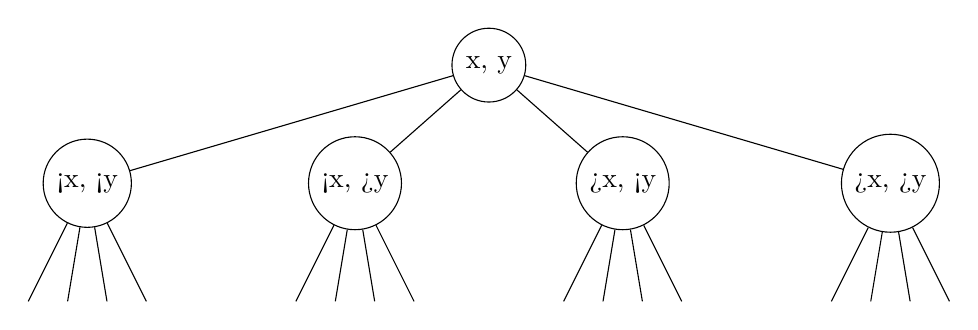
\begin{tikzpicture}
	[level 1/.style={sibling distance=34mm},
	level 2/.style={sibling distance = 5mm}]
	\tikzstyle{every node}=[circle,draw]
	\node {x, y}		
		child {
			node {<x, <y}
			child
			child
			child
			child
		}
		child {
			node {<x, >y}
			child
			child
			child
			child		
		}
		child {
			node {>x, <y}
			child
			child
			child
			child		
		}
		child {
			node {>x, >y}
			child
			child
			child
			child		
		}
	;
\end{tikzpicture}
	\caption{An illustration of the internal structure of the \texttt{Quadtree} data structure}
\end{figure}
\\
\subsubsection{FormatConverter class} % Converts from the data type pulled out of the data structure to the data type needed by the View package
The \texttt{FormatConverter} has static methods only, and only one public method. This methods takes an \texttt{ArrayList<Edge>} and converts it to the type \texttt{int[][][]} \\(\texttt{int[type][number of edges][edge coordinates]}).

The FormatConverter uses an instance of the Coordinates class to convert the given UTM32 coordinates to pixels as shown in the GUI.

\subsubsection{>>name<<DataCreator class}
These classes are not, strictly speaking, a part of the application (they are not used at runtime). They is a utility class, reading in the data supplied by Krak, writing it to the files \texttt{data.>>name<<}, optimized for building the data structures of the application.

\subsubsection{Graph class}
The \texttt{Graph} class actually contains two graph structures representing the road segments from Krak; one where the distances is the weight of the edges, and one where the time is the weight of the edges. These are used for finding the fastest and shortest paths respectively.
	
The static \texttt{Graph} object itself contains \texttt{ArrayList} representations of each of these graphs. These will be referred to as graphs from now on. The graphs contain \texttt{Vertex} objects which have a position, some neighbouring vertices, and some adjacent edges (of the type \texttt{GEdge}). A \texttt{HashMap} for each of these two graphs is used to quickly access a vertex, given its id. Two \texttt{HashMaps} are used since each graph has its representation of each edge (the edges have different weights across the graphs). When searching for a path, the correct \texttt{ArrayList} and \texttt{HashMap} are returned, depending on whether the user requests the fastest path of the shortest path.

Furthermore, a third \texttt{HashMap} is used to keep track of each \texttt{Vertex's} adjacent \texttt{GEdges}.

\subsubsection{Dijkstra}
The \texttt{Dijkstra} class contains the path finding algorithm used by our application. As the name of the class would suggest, this algorithm is Dijkstra's path finding algorithm. We chose to implement this algorithm because it is fairly simple and runs fast enough for our needs.